\chapter{ComCape}


\section{Übersicht}
Das ComCape, oder Communication Cape, ist eine zusätzliche Platine, welche sich auf den originalen BeagleBone Black oder auf das BeagleBone-Derivat stecken lässt. Ein Cape ist eine Platine, die eigens als Erweiterung für den BeagleBone entwickelt wurde. Solche Capes können den BBB zum Beispiel mit WLAN-Funktionalität erweitern und sind auch kommerziell erhältlich.

Das ComCape ist speziell für die Firma Variosystems entwickelt worden. Es erweitert den BBB, im Gegensatz zu den bereits erhältlichen Capes, um mehrere Funktionen:

\begin{itemize}
\item WLAN: Kabelloses Internet via Wireless LAN
\item GSM: Kabelloses Internet über das mobile Internet
\item BLE: Ermöglicht dem BBB eine drahtlose Verbindung über Bluetooth Low Energy
\item LCD: Über einen Flachbandstecker kann ein LCD mit kapazitivem Multi-Touch angeschlossen werden
\end{itemize}



\section{Allgemeiner Aufbau des ComCape}

\subsection{Elektrisches Schema}
Wie auch der BBB ist das ComCape auf 7 Top-Level Blätter verteilt:

\begin{itemize}
\item P01: Titelblatt
\item P02: WLAN 1/2
\item P03: WLAN 2/2
\item P04: GSM 1/2
\item P05: GSM 2/2
\item P06: BLE
\item P07: Stiftleiste und LCD-Stecker
\end{itemize}

Im Folgenden wird nur noch auf die Seitennummer des Schema (P01...P07) verwiesen, und nicht mehr auf den Namen.

Für alle nicht benutzten Pins der Bauteile wurden Testpunkte hinzugefügt, damit diese auch nachträglich noch zugänglich sind.

Alle Signale, die zum BBB führen, sind über einen 0$\Omega$ Widerstand geführt. So können alle Bauteile elektrisch vom BBB getrennt werden. Dies kann besonders nützlich sein, wenn ein Teil des ComCapes getrennt von dem Rest getestet werden will.

%Alle Designatoren von P02 starten mit 1, die von P03 mit 50, die Designatoren von P04 mit 100 u
%TODO Designatoren beschreiben

\section{Layout PCB}
Das PCB ist in drei Teile aufgeteilt. Auf dem unteren Teil befinden sich ausschliesslich Bauteile für das GSM, während der Mittlere Teil für WLAN-Bauteile reserviert ist. Im oberen Teil befinden sich neben dem Stecker für den LCD auch noch die Komponenten für das Bluetooth Modul.

Das Bluetooth-, das WLAN- und das GSM-Modul haben auch auf der Unterseite des ChipgehäuseS Pins, die gelötet werden müssen. Es ist nicht möglich, diese Bauteile von Hand zu löten. Aus diesem Grund wurden alle Bauteile auf der oberen Seite des PCBs im Reflow-Ofen gelötet. Für den Prototypenbau wurden die Bauteile auf der unteren Seite von Hand gelötet. Beim Erstellen des PCB-Layouts wurde darauf geachtet, dass möglichst viele Bauteile auf der oberen Seite platziert wurden. Zusätzlich wurde darauf geachtet, dass die linearen Spannungsregler, welche viel Abwärme produzieren, für die bessere Wärmeabgabe ebenfalls auf der oberen Seite platziert wurden. Die drei Module befinden sich ebenfalls auf der oberen Seite des PCBs.


\subsection{Grösse und Form des PCB}
Das ComCape sollte nicht grösser sein, als das LCD. Wenn man das LCD im Hochformat über das ComCape legt, ist das Cape aus diesem Grund gleich breit wie das LCD. Oben und unten wurde das Cape um je 1cm verlängert, um noch Befestigungsbohrungen platzieren zu können.

Da beim BBB die Ethernet-Buchse sehr hoch ist, hat das Cape auf der linken Seite eine Aussparung für diese Buchse. Zusätzlich ist die obere Hälfte des ComCapes schmaler, damit die Taster S1 und S3 vom BBB besser zugänglich sind. Anhang \ref{sec:anhang_befestigungsbohrungen} zeigt den Umriss des ComCapes und die Vermassung der Befestigungsbohrungen.



\section{Wirless LAN}
Für das Wireless LAN wurde das WL1835 Modul von Texas Instruments verwendet.

Für den BBB existiert bereits ein WLAN-Cape, welches gekauft werden kann. Auf diesem Cape ist ein WL1835 Modul verbaut. Das elektrische Schema und die Gerberdaten von diesem Cape sind frei erhältlich\cite{boardZooWLANCape}. Aus diesen Gründen haben wir das 'WL1835MOD W/ Chip Antenna' Cape als Referenzdesign verwendet.

%TODO Bild WLAN Cape


\subsection{Stromversorgung}
Die VDD\_3V3B Spannungsversorgung vom BBB wird für die prozessorseitige Spannungsversorgung des Spannungspegelwandlers verwendet.

Für die 3.3V-Spannungsversorgung wurde der gleiche lineare Spannungsregler verwendet, wie im Referenzdesign. Dieser Regler kann bis zu 1.5A liefern. Der effektive Strombedarf des Moduls ist abhängig vom Betriebsmodus und lässt sich nur schwer einschätzen. Deshalb wurde derselbe, vermutlich überdimensionierte, Spannungsregler wie im Referenzdesign verwendet. Der effektive Dauer- und Spitzen- Strom lässt sich im Betrieb mit einem Messwiderstand und einem Oszilloskop über dem Steckkontakt 'X1' messen.

Die 1.8V-Spannungsversorgung wird nur für die digitale Kommunikation verwendet. Aus diesem Grund wurde der 0.4A-Spannungsregler, welcher im Referenzdesign verwendet wird, mit einem 0.15A-Spannungsregler ersetzt, der auch in der Standardbibliothek von Variosystems zu finden ist. Auch bei dieser Versorgung lässt sich der effektive Strombedarf über den Steckkontakt 'X2' messen.

\subsection{Antenne}
Das ComCape unterstützt von der Hardware her zwei Antennen. In der Software wird aber nur eine unterstützt. Mehr dazu im Kapitel \ref{sec:wlan_varianten} weiter unten.

Bei der Antenne 1, welche gleichzeitig für WLAN und Bluetooth (ist in der Software nicht implementiert) genutzt wird, kann entweder die Kombination aus Chip- und PCB- Antenne oder eine externe Antenne verwendet werden. Wenn die externe Antenne verwendet werden soll, muss C54 eingelötet sein. Soll die PCB Antenne verwendet werden, muss C54 wieder ausgelötet und stattdessen C55 eingelötet werden.

Die externe Antenne kann über eine U.FL-Buchse angeschlossen werden.

Das PCB-Layout für die Chipantenne wurde aus dem Datenblatt der Chipantenne kopiert.

Für die Verbindung zwischen dem Modul und den Antennen wird eine Übertragungsleitung mit einer Wellenimpedanz vom 50$\Omega$ benötigt. Im Hardware User Guide von Telit[XXX] wird eine Übertragungsleitung mit den Massen, wie in Abbildung \ref{50OhmTransmissionLine} empfohlen. Berechnungen mit der Software 'txLine' haben gezeigt, dass sich die Wellenimpedanz nicht signifikant ändert, wenn diverse Masse, wie zum Beispiel die Dicke des PCB oder die Dielektrizitätskonstante des Dielektrikums, sich um 10\% ändern. Aus diesem Grund kann bei der Herstellung des PCB auf eine kontrollierte Impedanz verzichtet werden.

%TODO Quelle HW userguide Telit
%TODO Berechnungen

\begin{figure}[!ht]
\centering
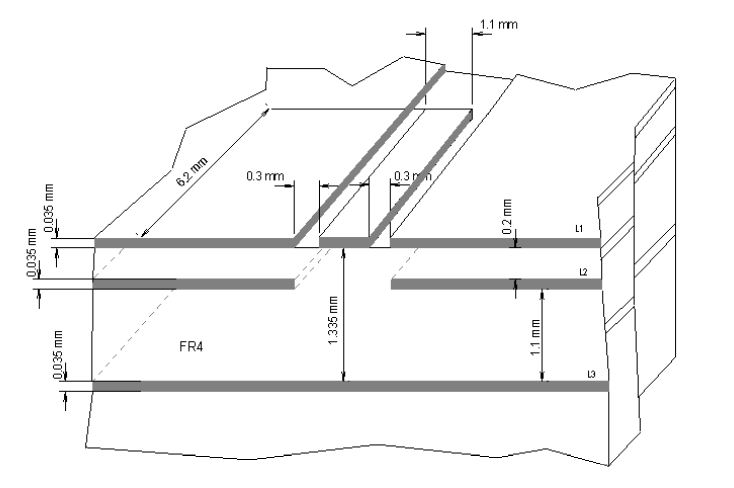
\includegraphics[angle=0,height=8cm]{images/50OhmTransmissionLine.jpg}
\caption{50$\Omega$ Übertragungsleitung}
\label{50OhmTransmissionLine}
\end{figure}


\subsection{32kHz Taktsignal}
Das Modul benötigt einen 32,768kHz Takt. Je nachdem, welche Widerstände eingelötet werden, können verschiedene Quellen für den Takt ausgewählt werden. Da bei der Planung des Capes nicht klar war, welche der Varianten funktionieren würde, sind alle drei Varianten auf dem Cape verwirklicht.

\textbf{R32: Lokaler Oszillator}: Der Oszillator erzeugt auf dem Cape einen 32kHz Takt und wird sonst nirgends verwendet. Dies ist die Standardvariante, da sie auch im Referenzdesign verwendet wird, und am wahrscheinlichsten funktioniert. Allerdings ist dieser Oszillator relativ teuer.

\textbf{R24: Von BBB erzeugt, mit Pegelwandler}: Diese Variante nutzt das Taktsignal, welches vom BBB erzeugt wird. Das 3.3V Signal wird dann mit einem TXS0108E auf 1.8V gewandelt. Ungünstiger weise wird dafür extra ein separater Pegelwandler benötigt.

\textbf{R28: Von BBB erzeugt, mit Spannungsteiler}: Auch diese Variante nutzt den Takt, der vom VBB erzeugt wird. Der Spannungspegel wird diesmal aber mit einem einfachen Spannungsteiler aus zwei Widerständen auf 1.8V gebracht. Das WLAN-Modul hat beim Eingang für dieses Taktsignal einen Eingangswiderstand von 1M$\Omega$\footnote{Quelle: Datenblatt WL1835MOD Seite 11}[XXX] und kann deshalb für diese Berechnung vernachlässigt werden. Wenn diese Variante funktioniert, ist sie am günstigsten und den anderen beiden vorzuziehen.
$$U_{out} =  3.3V * \dfrac{R29}{R29+R27} = 3.3V * \dfrac{4.7k\Omega}{4.7k\Omega+3.9k\Omega} = 1.80V$$

%TODO Quelle [XXX]

\subsection{Digitale Verbindung zum Prozessor}
Die WLAN-Daten werden über eienen SDIO Bus zum Prozessor übertragen. Der Spannungspegel wird dabei mit zwei TXS0108E Spannungswandlern von den 1.8V des Moduls auf 3.3V für den Prozessor gewandelt. Dieser Wandler funktioniert auf beide Richtungen, so dass auch Signale vom Prozessor zum WLAN-Modul auf den richtigen Pegel gewandelt werden.

Auf den zweiten TXS0108E kann verzichtet werden, wenn das 32kHz Taktsignal nicht vom VBB erzeugt wird.

\subsection{Varianten}\label{sec:wlan_varianten}
Das WL1835 Modul unterstützt neben einem Design mit zwei Antennen auch noch Bluetooth. Im ComCape wird Bluetooth und die zweite Antenne aber von der Software nicht unterstützt. Von der Hardware ist aber alles Nötige vorhanden. Die zweite Antenne könnte für MIMO oder eine MRC Konfiguration genutzt werden. MIMO steht für 'Multiple Input Multiple Output', damit kann im Vergleich zu einem Design mit einer Antenne (SISO = Single Input Single Output) die Bandbreite erhöht werden. Mit MRC oder 'Maximum Ratio Combining' kann die Reichweite des Signals erhöht werden.

Es existieren zum WL1835 pinkompatible Module, welche ein Design mit zwei Antennen, Bluetooth oder beides nicht unterstützen. In der Tabelle \ref{tab:wlanVarianten} sind alle vier Module und deren Funktionen aufgelistet.

\begin{table}

    \begin{tabular}{ | c | c | c | c | c |}
    \hline
    \textbf{Modul}		& \textbf{2.4-GHZ SISO}	& \textbf{2.4-GHZ MIMO}	& \textbf{2.4-GHZ MRC}	& \textbf{Bluetooth} \\ \hline
    
     WL1835MOD	& X				& X	 			& X				& X \\ \hline    
    
     WL1831MOD	& X				&	 			& 				& X \\ \hline  
    
     WL1805MOD	& X				& X	 			& X				&  \\ \hline  
    
     WL1801MOD	& X				& 	 			& 				&  \\ \hline  
    
    
    \end{tabular}
\caption{Varianten des WLAN Moduls}
\label{tab:wlanVarianten}
\end{table}


%TODO WAS NICHT FUNKTIONIERT UND WARUM


\section{GSM}


\subsection{Stromversorgung}
